\documentclass[11pt,pdftex,twoside,letterpaper]{exam}
\usepackage{amsmath,amssymb, amsthm}
%\usepackage{ccfonts,eulervm}
%\usepackage[T1]{fontenc}
\usepackage{graphicx}
\usepackage{xcolor}
\usepackage{booktabs}
\usepackage{caption}
\usepackage{setspace}
\usepackage[compact]{titlesec}
\usepackage{enumitem}
\usepackage{mdframed}
\usepackage[colorlinks=true,linkcolor=blue,citecolor=black,urlcolor=blue,bookmarks=false,pdfstartview={FitV}]{hyperref}
\usepackage{placeins}
\usepackage{cancel}
\usepackage{array}
\usepackage{float}
\usepackage{multirow}
\usepackage[many]{tcolorbox}
\usepackage{subcaption}

\newtcolorbox{mybox}[1]{%
    tikznode boxed title,
    enhanced,
    arc=0mm,
    interior style={white},
    attach boxed title to top center= {yshift=-\tcboxedtitleheight/2},
    fonttitle=\bfseries,
    colbacktitle=white,coltitle=black,
    boxed title style={size=normal,colframe=white,boxrule=0pt},
    title={#1}}


%%%%%%%%%%%%%%%%%%%%%%%%%%%%%%%%%%%%%%%%%%%%%%%%%%%%%%%%%%%%%%%%%%%%%%%%%%%%%
\renewcommand{\CancelColor}{\color{red}}

\DeclareRobustCommand{\bbone}{\text{\usefont{U}{bbold}{m}{n}1}}
\DeclareMathOperator{\EX}{\mathbb{E}}% expected value

%%%%%%%%%%%%%%%%%%%%%%%%%%%lists%%%%%%%%%%%%%%%%%%%%%%%%%%%%%%%%%%%%%%%%%%%%%%
%\setlist{nosep}        %no space anywhere --- too extreme for me
\setlist[description, 1]{itemsep=1ex}
\setlist[description]{topsep=0ex}
\setlist[itemize]{topsep=0ex}
\setlist[enumerate]{topsep=0ex, itemsep=0.0ex}
%%%%%%%%%%%%%%%%%%%%%%Margins%%%%%%%%%%%%%%%%%%%%%%%%%%%%%%%%%%%%%%%%%%%%%%%
\usepackage[top=1.25in, bottom=1.0in, left=1.0in, right=1.0in]{geometry}
\setlength{\parindent}{0in}
\setlength{\parskip}{\bigskipamount}
\raggedbottom

%titlesec definitions
\titlespacing*\section{0pt}{1pt plus 0pt minus 0pt}{0pt plus 0pt minus 0pt}
\titlespacing*\subsection{0pt}{1pt plus 0pt minus 0pt}{0pt plus 0pt minus 0pt}
\titlespacing*\subsubsection{0pt}{0pt plus 2pt minus 2pt}{0pt plus 2pt minus 2pt}

%%%%%%%%%%%%%%%%%%%%%%Headers and Footers%%%%%%%%%%%%%%%%%%%%%%%%%%%%%%%%%%
\pagestyle{headandfoot}
\runningheadrule
%\firstpageheadrule
% use "/" rather than the windows "\" in paths.
%\firstpageheader{}{}{\textbf{International Trade \&\\ Macroeconomics}\vspace{0.5cm}}
\runningheader{\textbf{Small open economy models}}{}{}
\runningfooter{}{}{\thepage}


%%%%%%%%%%%%%%%%%%%%%%%%%%%%%%%%%%%%%%%%%%%%%%%%%%%%%%%%%%%%%%%%%%%%%%%%%%%%%%%%%%%%%%%%%%%%%%%%%%%%%%%%%%%%%%%%%%%%%%%%%%%%%%%%%%%%
\begin{document}

\centerline{\Large Small open economy models}%
\smallskip
\centerline{This version: \today}


This note studies a class of models in which an economy has access to international borrowing and lending. We say the economy is small because it takes the interest rate and the prices of tradeable goods as given --- though not necessarily constant. A major focus of this literature is the behavior of the current account, which summarizes the borrowing and lending done in international markets.

We will begin with exchange models which are easier to characterize than models with production. First, we will tackle perfect foresight and then models with stochastic endowments. The goal is to understand how agents use external debt to smooth consumption and what this implies for the behavior of the current account and other variables of interest. We will then move on to models with production, which will usually require us to solve the models numerically.

\setcounter{section}{1}
\subsection{Perfect foresight exchange economy}

The country is populated by a representative consumer with preferences over sequences of consumption
\begin{equation}\label{eq:prefs}
  \sum_{t=0}^{\infty}\beta^t u\left(c_t\right)
\end{equation}
where $u$ is a well-behaved utility function and $\beta<1$ is the discount factor. The household faces a sequence of budget constraints of the form
\begin{equation*}
  c_t+b_{t+1} \leq \left(1+r \right)b_t+y_t  \qquad t=0,1,\ldots
\end{equation*}
with $b_0$ given and $c_t>0$. The household is endowed with tradeable goods $y_t$. In this section we assume that the sequence of $y$ is known. The beginning-of-period holdings of one-period bonds are $b_t$. Our notation implies that when $b_t<0$  the household is a net borrower from the rest of the world.

This framework allows us to define some often referenced concepts. The \textit{trade balance} or \textit{net exports} is
\begin{equation}\label{eq:tb-def}
  tb_t = y_t-c_t
\end{equation}
[What does $tb_t<0$ mean? $tb_t>0$?] When there is only one good in the economy, there cannot be both imports and exports in the economy. The \textit{current account} is the change in the country's net foreign asset position,
\begin{eqnarray}
% \nonumber % Remove numbering (before each equation)
  ca_t &=& b_{t+1}-b_t \\
     &=& y_{t} - c_t + rb_t\\
     &=& tb_t + rb_t
\end{eqnarray}
[To get to the second equality, solve the budget constraint for $b_{t+1}$.] The current account is the trade balance plus net capital income ($rb_t$). This definition implies that  unbalanced trade ($tb_t \neq 0$) is associated with a change in the net foreign asset position: either the country is borrowing from or lending to the rest of the world.

Our goal is to work out the consumption behavior of the household. It is easiest to do so with the lifetime budget constraint. The idea is to deflate the sequence budget constraint at $t$ by $(1+r)^t$ and then add them up. The first two terms are
\begin{eqnarray}
% \nonumber % Remove numbering (before each equation)
  c_0 + b_1 &=& (1+r)b_0 +y_0 \\
  \frac{c_1 +b_2}{1+r} &=& \frac{(1+r)b_1+y_1}{1+r}
\end{eqnarray}
Add these two equations and find
\begin{equation}\label{eq:lifetime-budget-step}
  c_0 +\frac{c_1}{1+r} +\frac{b_2}{1+r} = (1+r)b_0 + y_0 + \frac{y_1}{1+r}.
\end{equation}
Notice that $b_1$ cancels out and the beginning of a discounted sum of consumption and income are forming. If we continue in this way we find
\begin{equation}\label{eq:lifetime-budget}
  \sum_{t=0}^{\infty}\frac{c_t}{(1+r)^t} + \lim_{t \rightarrow \infty}\frac{b_{t+1}}{(1+r)^t} = \sum_{t=0}^{\infty}\frac{y_t}{(1+r)^t}+(1+r)b_0.
\end{equation}
The transversality condition says that $\lim_{t \rightarrow \infty}\frac{b_{t+1}}{(1+r)^t} =0$, and we have that the discounted value of consumption is equal to the households wealth, which is the discounted value of the endowment plus the beginning net foreign asset position.

We will maximize \eqref{eq:prefs} subject to \eqref{eq:lifetime-budget}. The Lagrangian is
\begin{equation}\label{eq:lagrangian}
  \Lambda = \sum_{t=0}^{\infty} \beta^t u\left(c_t\right) + \lambda \left(b_0(1+r) + \sum_{t=0}^{\infty}\frac{y_t-c_t}{(1+r)^t}\right)
\end{equation}
and the necessary first-order condition with respect to $c_t$ is
\begin{eqnarray}
  \beta^tu^\prime(c_t)&=&\frac{\lambda}{(1+r)^t}\\
  u^\prime(c_t)&=&\frac{\lambda}{[\beta(1+r)]^t}
\end{eqnarray}
The  solution sets the marginal utility of consumption equal to the marginal utility of a unit of wealth ($\lambda$) discounted by both the consumer's discount factor and the gross interest rate, which is the rate in which wealth grows if carried over a period.

Consumption behavior depends on $\beta(1+r)$. Assuming $u$ is well behaved, there are three possibilities
\begin{enumerate}
  \item $\beta(1+r)>1$ implies that $c_t\rightarrow \infty$. Relative to the rate of return, agents are patient. Accumulate assets and consume a lot in the future.
  \item $\beta(1+r)=1$ implies that $c_t = \bar{c}$. The household's patience exactly cancels out the return on saving.
  \item $\beta(1+r)<1$ implies that $c_t\rightarrow 0$. Agents are impatient relative to the rate of return, so they consume early.
\end{enumerate}

If we assume that $u(c) = \frac{c^{1-\sigma}}{1-\sigma} $ we can solve for $\lambda$,
\begin{eqnarray}
% \nonumber % Remove numbering (before each equation)
  c_t^{-\sigma} &=& \frac{\lambda}{[\beta(1+r)]^t}\\
  c_t &=& \lambda^{\frac{-1}{\sigma}}[\beta^{\frac{1}{\sigma}}(1+r)^{\frac{1}{\sigma}}]^t\\
  \sum \frac{c_t}{(1+r)^t} &=& \lambda^{\frac{-1}{\sigma}}\sum \frac{[\beta^{\frac{1}{\sigma}}(1+r)^{\frac{1}{\sigma}}]^t}{(1+r)^t}\\
  \sum \frac{y_t}{(1+r)^t} + (1+r)b_0 &=& \lambda^{\frac{-1}{\sigma}}\sum \frac{[\beta^{\frac{1}{\sigma}}(1+r)^{\frac{1}{\sigma}}]^t}{(1+r)^t}\\
  \sum \frac{y_t}{(1+r)^t} + (1+r)b_0 &=& \lambda^{\frac{-1}{\sigma}}\sum [\beta^{\frac{1}{\sigma}}(1+r)^{\frac{1-\sigma}{\sigma}}]^t\\
  Y &=& \lambda^{\frac{-1}{\sigma}}\sum [\beta^{\frac{1}{\sigma}}(1+r)^{\frac{1-\sigma}{\sigma}}]^t\\
  \frac{Y}{\sum [\beta^{\frac{1}{\sigma}}(1+r)^{\frac{1-\sigma}{\sigma}}]^t} &=& \lambda^{\frac{-1}{\sigma}}\\
  Y^{-\sigma} \left(\sum [\beta^{\frac{1}{\sigma}}(1+r)^{\frac{1-\sigma}{\sigma}}]^t\right)^{\sigma} &=& \lambda
\end{eqnarray}
If $Y$ is larger, the marginal value of wealth falls; The greater is $\sigma$ the greater is this effect. [As $\sigma$ increases, the agent is more risk averse.] We need $\beta^{\frac{1}{\sigma}}(1+r)^{\frac{1-\sigma}{\sigma}}<1$ for a solution to exist. Consumption is
\begin{equation}\label{eq:cons}
  c_t = Y \frac{[\beta^{\frac{1}{\sigma}}(1+r)^{\frac{1}{\sigma}}]^t}{\sum [\beta^{\frac{1}{\sigma}}(1+r)^{\frac{1-\sigma}{\sigma}}]^t}
\end{equation}
Suppose $\beta(1+r)=1$, so $\beta = 1/(1+r)$. The numerator on the right hand side is one and the denominator is $1/(r/(1+r))$, so consumption is $c_t=\frac{r}{1+r}Y$. Notice that consumption is constant, which we already knew.

Now we know about consumption. What does the path of consumption imply for borrowing and lending? Iterating backwards, the bond policy function is
\begin{eqnarray}
% \nonumber % Remove numbering (before each equation)
  b_{t+1} &=& tb_t+(1+r)b_t\\
   &=& \sum_{s=0}^{t} tb_s(1+r)^{t-s}+(1+r)^tb_0\\
   &=& (1+r)^tb_0+\sum_{s=0}^{t} (y_s-c_s)(1+r)^{t-s}\label{eq:b-backward}
\end{eqnarray}
which says that today's net foreign asset position is the discounted value of the initial position, plus the discounted value of all the previous trade balances, which keep track of the borrowing and lending done in the past. [Note that the trade balance plays the same role as the primary surplus in a fiscal policy setting.] We can also iterate forward on the budget constraint to find
\begin{eqnarray}
% \nonumber % Remove numbering (before each equation)
   b_{t+1} &=& \frac{b_{t+2}}{(1+r)}-\frac{tb_{t+1}}{(1+r)}\\
   &=& \lim_{s\rightarrow\infty} \frac{b_{t+s}}{(1+r)^{t+s-1}}-\sum_{s=0}^{\infty}  \frac{tb_{t+s}}{(1+r)^{t+s}}. \label{eq:b-forward}
\end{eqnarray}
This shows us that today's net foreign asset position (as long as there is no default) summarizes both the past and future borrowing and lending. For example: If the net foreign asset position is negative, it means that the country has consumed more than it was endowed in the past. It also means that the country must run trade surpluses in the future ($tb>0$).

The program \texttt{soe-deterministic.jl} computes an example in which output is constant at $y_L$ except for a brief period in which output is $y_H>y_L$. The results are plotted in Figure~\ref{fig:deterministic}. When $(1+r)\beta=1$ consumption will be constant and at a level above $y_L$. When the endowment is $y_L$, the trade balance is negative and net foreign asset position decreases. When the endowment switches to $y_H$, the trade balance is positive and the net foreign asset position becomes positive. Notice the difference between the current account and the trade balance after the endowment returns to $y_L$. The country finances its trade deficit with the return on its asset holdings.
\begin{figure}
  \centering
  \caption{Deterministic fluctuation in endowment}\label{fig:deterministic}
  \begin{subfigure}{0.49\textwidth}
    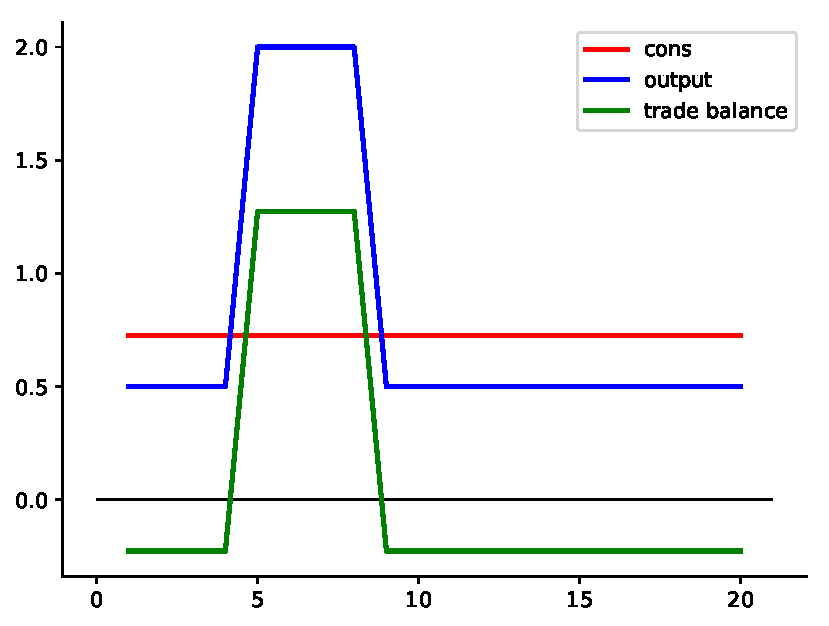
\includegraphics[width=\textwidth]{figures/cy.pdf}
    \caption{Output and consumption}
  \end{subfigure}
  \begin{subfigure}{0.49\textwidth}
    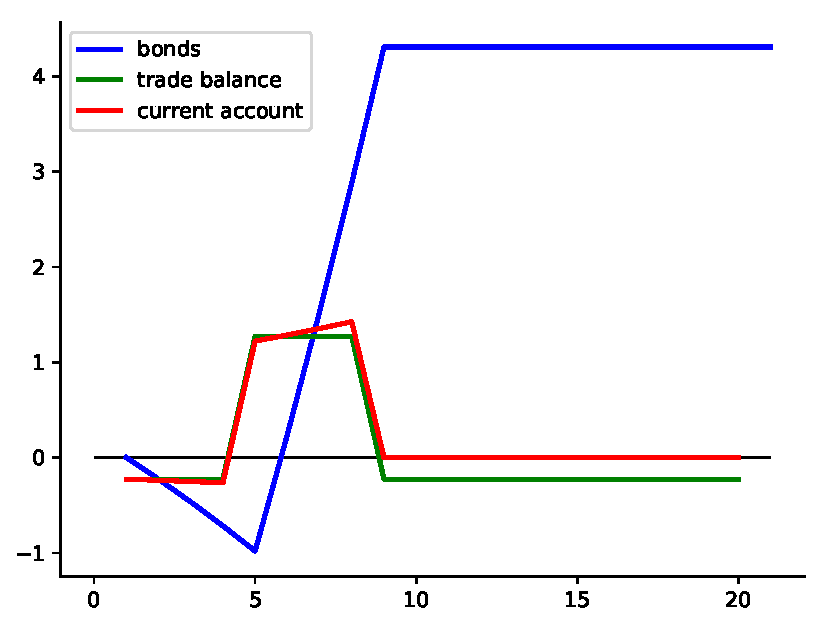
\includegraphics[width=\textwidth]{figures/debt.pdf}
    \caption{Current account and net foreign assets}
  \end{subfigure}
\end{figure}

\subsection{Stochastic exchange economy}
In this section we introduce uncertainty into our endowment economy. There are an infinite number of periods indexed by $t$. In each period an event $s_t$ occurs. The set of possible events at $t$ is $S_t$. Let the history of events that have occurred up to period $t$ be denoted $s^t=(s_0, s_1,\dots , s_t)$ and the probability that we have reached this history be $\pi(s^t)$. The set of histories that can occur at time $t$ is $S^t$. [If this notation confuses you, draw out the event tree. A history is one particular path (branch) from date 0 through date $t$.]


The uncertainty is over the endowment, $y(s^t)$. We will assume that the endowment follows an autoregressive process,
\begin{eqnarray}
% \nonumber % Remove numbering (before each equation)
  y(s^{t}) &=& \rho y(s^{t-1})+\epsilon(s^t) \label{eq:stoch-process}
\end{eqnarray}
where $\rho\in (0,1)$ and $\epsilon_t$ is an innovation process that is i.i.d. over time. [I guess we need that $y(s^{t-1})$ is large enough that we never have negative endowment?\footnote{Todo: with mean $\mu$ in the process, we have $y(s^{t+j})=\mu\frac{1-\rho^j}{1-\rho}+\rho^j y(s^t)$ and $c(s^t)=\frac{r}{1+r}\sum_{t=0}^{\infty} \left( \frac{\mu}{1-\rho}\frac{1-\rho^j}{(1+r)^j}+\left(\frac{\rho}{1+r}\right)^j y(s^t)\right)+rb(s^t)$. Need to double check and work out.} ]
To make our lives simple, let $u(c_t)=-\frac{1}{2}\left(c_t - \bar{c}\right)^2$. The household's problem is now
\begin{equation}
 \max_{c(s^t),b(s^{t+1})} \;\; -\sum_{t=0}^\infty \sum_{s^t\in S^t} \pi(s^t) \beta^t\frac{1}{2}\left(c(s^t) -\bar{c}\right)^2
\end{equation}
\begin{equation}
  \textrm{s.t.}\;\; c(s^t)+b(s^{t+1}) \leq  (1+r)b(s^t) +y(s^t)\qquad \forall s^t\in S^t
\end{equation}
with $b_0$ given and $\bar{c}\geq c(s^t)\geq0$. The first order conditions are, for each $s^t$,
\begin{eqnarray}
% \nonumber % Remove numbering (before each equation)
  -\pi(s^t)\beta^t \left(c(s^t) -\bar{c}\right) &=& \lambda(s^t)\\
  \lambda(s^t)& =& (1+r) \sum_{s^{t+1}} \lambda(s^{t+1}).
\end{eqnarray}
Combining the first order conditions,
\begin{eqnarray}
   \pi(s^t)\beta^t \left( c(s^t) -\bar{c} \right)&=& (1+r)\sum_{s^{t+1}}\pi(s^{t+1})\beta^{t+1} \left( c(s^{t+1}) -\bar{c}\right)\\
   c(s^t)&=& (1+r)\beta\sum_{s^{t+1}}\pi(s^{t+1}|s^t) c(s^{t+1}).
\end{eqnarray}
With $(1+r)\beta=1$, consumption is a random walk,
\begin{equation}
  c(s^t)=\EX_tc(s^{t+1})
\end{equation}
As in the deterministic model, we can iterate on the budget constraint. After $k$ iterations we have
\begin{eqnarray}
   b(s^{t}) &=& \frac{b(s^{t+k})}{(1+r)^k}-\sum_{j=0}^k\frac{tb(s^{t+j})}{(1+r)^{j+1}}.
\end{eqnarray}
Take the time-$t$ expectation and  then the limit as $k\rightarrow\infty$, to yield
\begin{eqnarray}
% \nonumber % Remove numbering (before each equation)
   b(s^t) &=& -\EX_t\sum_{j=0}^k\frac{tb(s^{t+j})}{(1+r)^{j+1}}.
\end{eqnarray}
[This requires that $\lim_{j\rightarrow \infty}\EX_t\frac{b(s^{t+j})}{(1+r)^{t+j}}=0$.] The intuition is the same: the value of today's net foreign asset position is equal to the discounted expected value of future trade surpluses. Substitute the definition of the trade balance and rearrange to form (note that I pulled a $1+r$ term out of the summations)
\begin{eqnarray}
% \nonumber % Remove numbering (before each equation)
   b(s^t) &=& -\frac{1}{1+r}\EX_t\sum_{j=0}^k\frac{y(s^{t+j})}{(1+r)^{j}} + \frac{1}{1+r}\EX_t\sum_{j=0}^k\frac{c(s^{t+j})}{(1+r)^{j}}. \label{eq:lom-b-stochastic}
\end{eqnarray}
Swap the summation for the expectation and the consumption term is
\begin{eqnarray}
% \nonumber % Remove numbering (before each equation)
  \EX_tc(s^t) +\frac{\EX_tc(s^{t+1})}{(1+r)}+\frac{\EX_tc(s^{t+2})}{(1+r)^2}+\dots
\end{eqnarray}
and since consumption is a random walk (apply iterated expectations), the consumption term is just
\begin{equation}
  \frac{1}{1+r}\EX_t\sum_{j=0}^k\frac{c(s^{t+j})}{(1+r)^{j}} = \frac{1}{r}c(s^t).
\end{equation}
Substitute this into \eqref{eq:lom-b-stochastic} and solve for $c(s^t)$,
\begin{eqnarray}
% \nonumber % Remove numbering (before each equation)
   rb(s^{t}) + \frac{r}{1+r}\EX_t\sum_{j=0}^k\frac{y(s^{t+j})}{(1+r)^{j}}&=& c(s^t).
\end{eqnarray}
The household consumes a constant share of its \textit{expected} wealth, which is made up of the its net asset position and the expected value of its endowment.

We still have $y(s^t)$ to deal with. From \eqref{eq:stoch-process} and the law of iterated expectations, we have $\rho^jy(s^t)=\EX_{t}y(s^{t+j})$. Use this to get rid of the sum,
\begin{eqnarray}
% \nonumber % Remove numbering (before each equation)
    c(s^t)&=&rb(s^{t}) + \frac{r}{1+r}\sum_{j=0}^\infty\frac{\EX_ty(s^{t+j})}{(1+r)^{j}}\\
   c(s^t)&=&rb(s^{t}) + \frac{r}{1+r}\sum_{j=0}^\infty\frac{\rho^jy(s^{t})}{(1+r)^{j}}\\
   c(s^t)&=&rb(s^{t}) + \frac{r}{1+r}y(s^{t})\sum_{j=0}^\infty\frac{\rho^j}{(1+r)^{j}}\\
   c(s^t)&=&rb(s^{t}) + y(s^{t}) \frac{r}{1+r-\rho}.
\end{eqnarray}
So now we have the consumption as a function of the current endowment and last period's net foreign asset position. Since $\rho\in(-1,1)$, the coefficient on $y(s^t)$ is always less than one. Consumption responds less than output --- this is consumption smoothing. We will discuss the dependence on $\rho$ shortly. The other variables of interest are
\begin{eqnarray}
% \nonumber % Remove numbering (before each equation)
  tb(s^t) &=& y(s^t)-c(s^t) =  y(s^{t}) \frac{1-\rho}{1+r-\rho}-rb(s^{t})\\
  ca(s^t) &=& tb(s^t)+rb(s^t) = y(s^{t}) \frac{1-\rho}{1+r-\rho} \label{eq:ca-stationary}\\
  b(s^{t+1}) &=& b(s^t) + ca(s^t) = b(s^t) + y(s^{t}) \frac{1-\rho}{1+r-\rho}.
\end{eqnarray}
External debt follows a random walk (the coefficient on $b(s^t)$ is one). The behavior of the model depends on the persistence of the endowment process, which is governed by $\rho$. Consider an innovation to the endowment, $\epsilon(s^t)$.
\begin{enumerate}
  \item Temporary shocks, $\rho=0$. Since $rb(s^t)$ is already determined at time $t$, consumption changes according to $\Delta c(s^t) = \frac{r}{1+r}\epsilon(s^t)$. This is a purely transitory shock, so consumption does not change much --- the shock gets smoothed. The current account absorbs most of the shock,
      \begin{equation}
        ca(s^t)=\frac{1}{1+r}[0\times y(s^{t-1})+\epsilon(s^t)]=\epsilon(s^t)\frac{1}{1+r},
      \end{equation} and $b(s^{t+1}) = b(s^t) + \epsilon(s^t)\frac{1}{1+r}$. If the shock is negative, the net asset position decreases and the household borrows to smooth consumption. The current account is procyclical and about as volatile as output, $\sigma(c)=\frac{r}{1+r}\sigma(y)$.
      \item Almost permanent shocks, $\rho \rightarrow 1$. Since $rb(s^t)$ is already determined at time $t$, consumption changes according to $\Delta c(s^t) = \epsilon(s^t)$. This is a ``permanent'' change in income, so you consume it. This means that the household does not adjust its savings so $ca_(s^t)=0$ and $tb(s^t)=-rb(s^t)$. The current account is acyclical and is less volatile (duh) than output.
      \item Persistent, but not permanent shocks, $\rho\in(0,1)$. Shocks mean revert. Suppose $\epsilon(s^t)>0$. Consumption jumps up, but by less than the shock. While output is ``high'' we have $ca(s^t)>0$ and the country's net foreign asset position increases. After the shock has decayed away, the country finances the increases consumption through the return on its savings, $\Delta c = r \Delta b$. The impulse response functions are plotted in Figure~\ref{fig:stochastic-endowment}.
\end{enumerate}
The program \texttt{soe-random.jl} computes the equilibrium of this model. It is useful to experiment with different values of $\rho$ in the program to get a feel for how the persistence of the output process affects the current account.
\begin{figure}
  \centering
  \caption{Impulse response in the stochastic endowment model ($r=0.05$ and $\rho=0.8$).}\label{fig:stochastic-endowment}
  \begin{subfigure}{0.49\textwidth}
    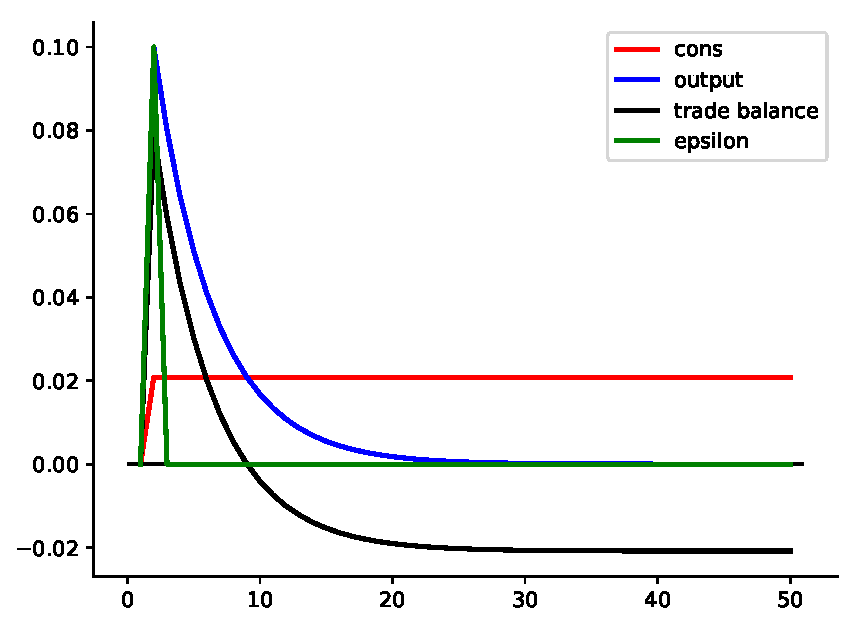
\includegraphics[width=\textwidth]{figures/cy_st.pdf}
    \caption{Output and consumption}
  \end{subfigure}
  \begin{subfigure}{0.49\textwidth}
    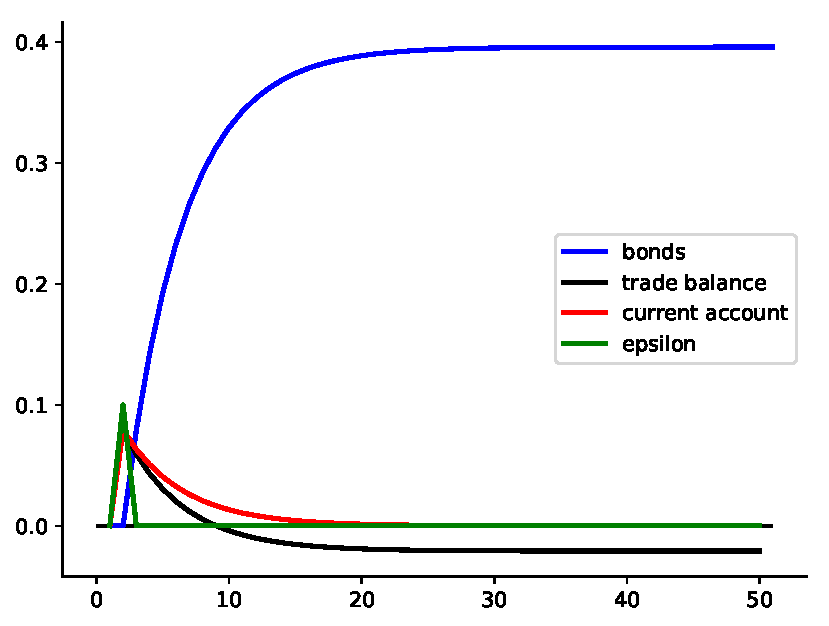
\includegraphics[width=\textwidth]{figures/debt_st.pdf}
    \caption{Current account and net foreign assets}
  \end{subfigure}
\end{figure}



\subsubsection{Nonstationary endowment} \label{sec:nonstationary-shocks}
In this section we introduce shocks to the growth rate of the endowment process.
\begin{eqnarray}
% \nonumber % Remove numbering (before each equation)
  \Delta y(s^t) &=& \rho \Delta y(s^{t-1}) + \epsilon(s^t)\\
  y(s^t) &=& y(s^{t-1})+\rho \Delta y(s^{t-1}) + \epsilon(s^t)
\end{eqnarray}
where $\epsilon \sim N(0,\sigma^2_\epsilon)$ and $\rho \in [0,1)$. A feature of this specification is that a one-time shock from $\epsilon$ has a permanent effect on the level of future income. To see this, suppose that $\epsilon(s^t)>0$ and, for all $j=0,1,\ldots$, $\epsilon(s^{t+j})=0$.  For simplicity, assume that $\Delta y(s^{t-1})=0$.
\begin{eqnarray}
  y(s^{t+1}) &=& y(s^{t})+\rho \Delta y(s^{t}) + \epsilon(s^{t+1})
\end{eqnarray}
since $\epsilon(s^{t+1})=0$
\begin{eqnarray}
  y(s^{t+1}) &=& y(s^{t})+\rho \Delta y(s^{t})
\end{eqnarray}
and $\Delta y(s^t) = \rho \Delta y(s^{t-1}) + \epsilon(s^t)$
\begin{eqnarray}
  y(s^{t+1}) &=& y(s^{t})+\rho \left[ \rho \Delta y(s^{t-1}) + \epsilon(s^t) \right]
\end{eqnarray}
with $\Delta y(s^{t-1})=0$
\begin{eqnarray}
  y(s^{t+1}) &=& y(s^{t})+\rho \left[ \rho  + \epsilon(s^t) \right]
\end{eqnarray}
 $y(s^t) = y(s^{t-1})+\rho \Delta y(s^{t-1}) + \epsilon(s^t)$
\begin{eqnarray}
  y(s^{t+1}) &=& y(s^{t-1}) + \epsilon(s^t)+ \rho\epsilon(s^t), \; \textrm{and similarly},\\
  y(s^{t+2}) &=& y(s^{t-1}) + \epsilon(s^t)+ \rho\epsilon(s^t) + \rho^2\epsilon(s^t)\\
  \lim_{j \to \infty} y_{t+j} &=& y(s^{t-1}) + \frac{1}{1-\rho}\epsilon(s^t)
\end{eqnarray}
Since $\epsilon(s^t)$ has mean zero, this is also true in expectation.

We haven't changed anything about the environment besides the shock process, so the first order conditions, etc. are the same as in the model with stationary shocks. Like we did before, lets work out the solution to the model, focusing on the behavior of the current account. As before, consumption  and the current account are
\begin{eqnarray}
  c(s^t) &=& rb(s^t) + \frac{r}{1+r}\sum_{j=0}^\infty\frac{\EX_ty(s^{t+j})}{(1+r)^j}\\
  ca(s^t) &=& y(s^t)-c(s^t)+rb(s^t).
\end{eqnarray}
Substitute consumption into the current account definition, then peel off the $t=0$ term in the sum and combine it with the $y(s^t)$ term
\begin{eqnarray}
  ca(s^t) &=& y(s^t) - \frac{r}{1+r}\sum_{j=0}^\infty\frac{\EX_ty(s^{t+j})}{(1+r)^j} \\
  ca(s^t) &=& \frac{1}{1+r}y(s^t) - \frac{r}{1+r}\sum_{j=1}^\infty\frac{\EX_ty(s^{t+j})}{(1+r)^j}
\end{eqnarray}
break the summation up into
\begin{eqnarray}
  ca(s^t) &=& \frac{1}{1+r}y(s^t) - \sum_{j=1}^\infty\frac{\EX_ty(s^{t+j})}{(1+r)^j}+ \frac{1}{1+r}\sum_{j=1}^\infty\frac{\EX_ty(s^{t+j})}{(1+r)^j}\\
  ca(s^t) &=& - \sum_{j=1}^\infty\frac{\EX_ty(^{t+j})}{(1+r)^j}+ \frac{1}{1+r}\sum_{j=0}^\infty\frac{\EX_ty(s^{t+j})}{(1+r)^j}\\
  ca(s^t) &=& - \sum_{j=1}^\infty\frac{\EX_ty(s^{t+j})}{(1+r)^j}+ \sum_{j=1}^\infty\frac{\EX_ty(s^{t+j-1})}{(1+r)^j}\\
  ca(s^t) &=& - \sum_{j=1}^\infty\frac{\EX_t \Delta y(s^{t+j})}{(1+r)^j}.
\end{eqnarray}
Given our specification of the endowment, we have $\EX_t\Delta y(s^{t+j})=\rho^j\Delta y(s^t)$. Use in the above equation to yield
\begin{eqnarray}
  ca(s^t) &=& - \sum_{j=1}^\infty\frac{\rho^j \Delta y(s^t)}{(1+r)^j}\\
  ca(s^t) &=& - \Delta y(s^t)\sum_{j=1}^\infty\left(\frac{\rho }{1+r}\right)^j\\
  ca(s^t) &=& - \frac{\rho }{1+r-\rho}\Delta y(s^t).
\end{eqnarray}
Compare this to the current account behavior in the model with stationary shocks \eqref{eq:ca-stationary}. The signs are flipped --- this model is qualitatively different than the model that is identical in every way except for the shock process. The intuition is simple. Suppose the economy is hit with a positive innovation to the endowment
\begin{itemize}
  \item In the model with a stationary output process, the shock means that output will be \textbf{temporarily} higher. The optimal thing to do is save some of it (how much depends on the persistence of the process) and spread the temporary increase across time.
      \[
      ca(s^t)  = y(s^{t}) \frac{1-\rho}{1+r-\rho}
      \]
  \item In the model with a nonstationary output process, the innovation means that output will be permanently higher. The optimal thing to do is to borrow today against the future income increase. Again, this depends on $\rho$.
      \[
      ca(s^t) = - \frac{\rho }{1+r-\rho}\Delta y(s^t)
      \]
\end{itemize}
We have the current account, so now work out the consumption process. Start by differencing the definition of the current account, then solve for consumption growth.
\begin{eqnarray}
% \nonumber % Remove numbering (before each equation)
  ca(s^t)-ca(s^{t-1}) &=& \Delta y(s^t)-\Delta c(s^t)+r\left[b(s^t)-b(s^{t-1})\right]\\
   \Delta c(s^t) &=& \Delta y(s^t)+r\left[b(s^t)-b(s^{t-1})\right]-\left[ca(s^t)-ca(s^{t-1})\right]
\end{eqnarray}
Now take another definition of the current account $ca(s^{t-1})=b(s^{t})-b(s^{t-1})$ and write
\begin{eqnarray}
% \nonumber % Remove numbering (before each equation)
  \Delta c(s^t) &=& \Delta y(s^t)+r\left[ca(s^{t-1})\right]-\left[ca(s^t)-ca(s^{t-1})\right]\\
  \Delta c(s^t) &=& \Delta y(s^t)-ca(s^{t}) + (1+ r) ca(s^{t-1})
\end{eqnarray}
substitute the solutions for the current accounts
\begin{eqnarray}
% \nonumber % Remove numbering (before each equation)
  \Delta c(s^t) &=& \Delta y(s^t)+\frac{\rho}{1+r-\rho}\Delta y(s^t) - \frac{(1+r)\rho}{1+r-\rho}\Delta y(s^{t-1})\\
  \Delta c(s^t) &=& \frac{1+r}{1+r-\rho}\Delta y(s^t) - \frac{(1+r)\rho}{1+r-\rho}\Delta y(s^{t-1}) \\
  \Delta c(s^t) &=& \frac{1+r}{1+r-\rho} \left[\rho \Delta y(s^{t-1}) + \epsilon(s^t) \right] - \frac{(1+r)\rho}{1+r-\rho}\Delta y(s^{t-1})\\
  \Delta c(s^t) &=& \frac{1+r}{1+r-\rho}\epsilon(s^t) \label{eq:cons-nonstationary}
\end{eqnarray}
How does the behavior the economy change with $\rho$?
\begin{enumerate}
  \item When $\rho = 0$, the income level is a random walk and income and consumption move one-for-one, $\Delta c(s^t)=\epsilon(s^t)$ (see equation \ref{eq:cons-nonstationary}) and the current account doesn't change, $ca(s^t)=0$. This is the same as the case in which $\rho\rightarrow 1$ in the stationary income model.
  \item When $\rho>0$, income is stationary in first-differences. Consumption growth rates move more than one-for-one with income growth rates. Suppose $r=0.04$ and $\rho=0.5$. Then $\Delta c = 1.93 \epsilon$
\end{enumerate}
When turning to the data, we will often look at second moments. (The data are usually made stationary through some kind of filter.) In this model we have\footnote{Reminder (for me, mostly): $\sigma^2(y_t)=\rho^2 \sigma^2(y_{t-1}) + \sigma^2(\epsilon_2)$ means that $\sigma(y) = \sigma(\epsilon)/\sqrt{1-\rho^2}$.}
\begin{eqnarray}
% \nonumber % Remove numbering (before each equation)
  \sigma(\Delta c) &=& \frac{1+r}{1+r-\rho}\sigma(\epsilon)\\
  \sigma(\Delta c) &=& \frac{1+r}{1+r-\rho}\sqrt{1-\rho^2}\sigma(\Delta y)
\end{eqnarray}
where the second line follows from the $\epsilon$ shocks being normal: $\sigma^2(\Delta y) = \frac{\sigma^2(\epsilon)}{1-\rho^2}$.

\subsection{Data}

The classic approach to business cycle analysis is to use the first moments of the data to calibrate or estimate the model and to compare the model's second moments to the second moments in the data. If the model can replicate the second moments in the data, the model is considered successful. In general, the idea is to use one set of moments (first or otherwise) to parameterize the model and a different set of moments to get a sense of model fit.

 Business cycle data --- international or otherwise --- is typically made stationary before computing second moments. There are several ways to ``detrend'' the data by extracting a cyclical component $y^c_t$ and a smoothed component, or a trend component, $y^s_t$.
 \begin{enumerate}
   \item First differences. $y_t^c = y_t-y_{t-1}$. Simple. Consistent with model in section~\ref{sec:nonstationary-shocks}.
   \item The Hodrick-Prescott filter. Very popular. A smoothing parameter controls the frequency of the extracted cycle. Not great if end points are not on trend. Let $y_t = y^s_t+y^c_t$.
       \begin{equation}
         \min_{y_t^s} \;\; \sum_{t=1}^T \left(y^s_t-y_t \right)^2 + \lambda\sum_{t=2}^T \left[ \left( y_{t+1}^s-y_t^s \right) - \left( y_{t}^s-y_{t-1}^s \right) \right]^2
       \end{equation}
       The smoothing parameter $\lambda$, determines the amount of nonlinearity in the trend component. As $ \lambda \to \infty$, the trend is linear. If $\lambda=0$ the trend is the data. Hodrick and Prescott liked $\lambda=1600$ for quarterly data and $\lambda=100$ for annual data. Ravn and Uhlig (2002) suggest 6.25 for annual data.
   \item Band-pass filters. Taken from signal processing. It passes business cycles of certain frequencies and rejects longer or shorter business cycles.
   \item Regressions on time trends.
 \end{enumerate}

 First differences and the HP filter are popular. Band-pass filters used to be more popular. People argue a lot about how to detrend data and much has been said about the HP filter. Despite papers such as ``Why you should never use the Hodrick-Prescott filter,'' it remains a very popular way to approach the data.

The standard operating procedure for generating business cycle moments using the HP filter:
\begin{enumerate}
  \item Take logs of the data: $\left\{y_t\right\}\rightarrow \left\{\log y_t\right\}$
  \item Apply the HP filter using your favorite statistical package to yield $\left\{y^s_t, y^c_t\right\}$. Note that since the data are in logs, the cyclical component is a percent deviation from the trend component.
  \item Compute moments from $\left\{y^c_t\right\}$, e.g., $\sigma\left(y^c_t\right)$
\end{enumerate}
For variables that can be negative (the trade balance, current account) do not take logs. Instead, express them as shares of GDP, then continue at step 2.

\begin{table}[H]
  \centering
  \caption{Business cycle second moments}\label{tab:moments}
  \begin{tabular*}{\textwidth}{l@{\extracolsep{\fill}}cccc}
  \toprule
    & $\sigma(y)$     &      $ \sigma\left(\frac{tb}{y}\right)$        &  $ \rho\left(\frac{tb}{y}\right)$     &$ \frac{\sigma(c)}{\sigma(y)}$\\
    \midrule
    Industrialized  & 1.34  &1.02   &--0.17                 &0.94\\
    Emerging        & 2.74      & 3.22      & --0.51        & 1.45\\
  \bottomrule
  \end{tabular*}
\end{table}
The data are from Aguiar and Gopinath (2007). Note that the trade balance has been used instead of the current account. The two are very similar for most countries, and data on the trade balance is much easier to obtain, especially for emerging economies. How are ``rich'' and ``poor'' countries different?
\begin{enumerate}
  \item Output is more volatile in emerging markets.
  \item The trade balance is more volatile and more counter-cyclical in emerging markets.
  \item Consumption is more volatile than output in emerging markets.
\end{enumerate}

\subsection{Two goods and relative prices} [todo: add $s^t$ notation; clean up; bonds denominated in foreign goods]

\subsubsection{Preliminaries}
Consumption is made up of two goods, $c_m$ and $c_x$, the import and export good,
\begin{eqnarray}
% \nonumber % Remove numbering (before each equation)
  c_t &=& \left(c_{mt}^\frac{\gamma-1}{\gamma}+\tau^\frac{1}{\gamma}c_{xt}^\frac{\gamma-1}{\gamma}\right)^\frac{\gamma}{\gamma-1}.
\end{eqnarray}
The country is endowed with the export good, and its price, $p_x$, is exogenous and stochastic. Normalize $p_m=1$. This introduces the concept of the \textit{terms of trade},
\begin{eqnarray}
% \nonumber % Remove numbering (before each equation)
  tot_t &=& \frac{p_{xt}}{p_{mt}},
\end{eqnarray}
but be careful --- some people define the terms of trade as $p_m/p_x$.  The price of a unit of the consumption good solves
\begin{equation}
    P_t = \min_{c_x, c_m} \;\; p_{xt} c_{xt} + c_{mt}\\
\end{equation}
 \begin{eqnarray}
 \textrm{s.t.}\;\; 1& =\left(c_{mt}^\frac{\gamma-1}{\gamma}+\tau^\frac{1}{\gamma}c_{xt}^\frac{\gamma-1}{\gamma}\right)^\frac{\gamma}{\gamma-1}
\end{eqnarray}
which is
\begin{eqnarray}
% \nonumber % Remove numbering (before each equation)
  P_t = \left(1+\tau p_{xt}^{1-\gamma}\right)^\frac{1}{1-\gamma}.
\end{eqnarray}
Now we have potentially differing consumption prices in the home country and the rest of the world [e.g., suppose the weights on $m$ and $x$ goods differ in the consumption aggregator]. Let $P^*$ be the price of consumption in the rest of the world and $e$ be the foreign currency cost of one unit of the home currency. The \textit{real exchange rate} is defined as
\begin{eqnarray}
% \nonumber % Remove numbering (before each equation)
  rer_t &=& e_{t}\frac{P_t}{P_t^*}. \qquad \textrm{In what units is the rer?} \\
  \textrm{rer units} & = & \frac{\textrm{dollars}}{\textrm{peso}} \frac{\textrm{pesos / home basket}}{\textrm{dollars/ row basket}}=\frac{\textrm{row basket}}{\textrm{home basket}}
\end{eqnarray}
An increase in the real exchange rate is an appreciation of the home currency and a depreciation of the foreign currency --- it now takes more foreign baskets to purchase one home basket.

The bond is denominated in units of SOE consumption basket. The household budget constraint at time $t$ is
\begin{eqnarray}
% \nonumber % Remove numbering (before each equation)
  p_{xt} c_{xt} + c_{mt} +P_tb_{t+1} &=& p_{xt}y_t+(1+r)P_tb_t \qquad \textrm{or}\\
  P_tc_{t} +P_tb_{t+1} &=& p_{xt}y_t+(1+r)P_tb_t\\
  c_{t} +b_{t+1} &=& \frac{p_{xt}}{P_t}y_t+(1+r)b_t
\end{eqnarray}
The nominal trade balance is
\begin{eqnarray}
% \nonumber % Remove numbering (before each equation)
  tb_t &=& p_{x,t}(y_t-c_{x,t})-c_{m,t} = p_{x,t}y_t-P_tc_t
\end{eqnarray}
where the last line follows because $p_xc_x + p_mc_m=Pc$. This is the nominal trade balance because it has fluctuating prices in it. The current account is
\begin{eqnarray}
% \nonumber % Remove numbering (before each equation)
  b_{t+1} -b_t &=& \frac{p_{xt}}{P_t}y_t- c_t+rb_t \\
  b_{t+1} -b_t &=& \frac{tb_t}{P_t}+rb_t
\end{eqnarray}
Notice that the trade balance is expressed in the units of consumption goods that it can provide. This makes sense, since the bonds are denominated in units of the home consumption basket.

\subsubsection{Model}
\begin{equation}
 \max_{c(s^t),b(s^{t+1})} \;\; \sum_{t=0}^\infty \sum_{s^t\in S^t} \pi(s^t) \beta^tu(c(s^t))
\end{equation}
\begin{eqnarray}
% \nonumber % Remove numbering (before each equation)
  \textrm{s.t.} \; c_{t} +b_{t+1} &=& \frac{p_{xt}}{P_t}y_t+(1+r)b_t \qquad \forall s^t
\end{eqnarray}
along with the usual no-Ponzi, transversality, etc.
In this case, fluctuations in the quantity of the endowment and fluctuations in the \textbf{value of the endowment in terms of consumption}, $p_x/P$ generate income fluctuations.

\begin{mybox}{Special case}
Assume that the exported good is not consumed, only the imported good is consumed. Since $p_m(s^t)=1$ then $P(s^t)=1$.  Assume that the endowment is constant $y(s^t)=1$ and that $(1+r)\beta=1$. The utility function is $u(c)=-(c_t-\bar{c})^2\frac{1}{2}$. Further, assume that
\begin{eqnarray}
% \nonumber % Remove numbering (before each equation)
  tot(s^t) &=& \rho \; tot(s^{t-1}) + \epsilon(s^t)
\end{eqnarray}

Now the country is responding to terms-of-trade shocks that change its income. The we have, as before,
\begin{eqnarray}
% \nonumber % Remove numbering (before each equation)
  b(s^t) &=& -\EX_t \sum_{j=0}^\infty\frac{tot(s^{t+j})-c(s^{t+j})}{(1+r)^{j+1}}
\end{eqnarray}
All of our previous analysis goes through as before. And the relationship between the current account and the terms of trade is
\begin{eqnarray}
% \nonumber % Remove numbering (before each equation)
  ca(s^t) &=&   \frac{1-\rho}{1+r-\rho} tot(s^{t})
\end{eqnarray}
This relationship implies that an increase in the terms of trade should lead to an increase in the current account. As before, the more persistent is the shock, the less the impact should be on the current account. This relationship was studied in Obstfeld (1982) and Svensson and Razin (1983). [USG book covers this in more detail in section 7.3.2.]
\end{mybox}

\section{Production}
Production models will generally be too difficult to solve analytically. The usual way forward is to use local approximations to the model equilibrium, which raises the question: ``Local approximation around what?'' A natural point would be the steady state, but our models do not have a steady state that is not history dependent. Lets start with a deterministic model.
\begin{equation}
 \max_{c,b_{t+1}, i_t, k_{t+1}} \;\; \sum_{t=0}^\infty  \beta^tu(c_t)
\end{equation}
\begin{eqnarray}
% \nonumber % Remove numbering (before each equation)
  \textrm{s.t.} \; c_{t} +b_{t+1} +i_t &=& z_tk_t^\alpha+(1+r)b_t\\
  k_{t+1}&=& k_t(1-\delta)+i_t
\end{eqnarray}
Here we have introduced capital $k$ and investment $i$. The production function is $y=zk^\alpha$ and $z$ will vary over time in a deterministic way. Let $\lambda_t$ be the multiplier on the budget constraint and $\mu_t$ be the multiplier on the law of motion for capital. [The multiplier $\mu$ is the benefit from a marginal increase in the capital stock. Maybe a better notation is $q$.] The first order conditions are
\begin{eqnarray}
% \nonumber % Remove numbering (before each equation)
  c_t:&u'(c_t)\beta^t = \lambda_t\\
  i_t: &\lambda_t=\mu_t\\
  b_{t+1}:&\lambda_t=(1+r)\lambda_{t+1}\\
  k_{t+1}:&\mu_t=(1-\delta)u_{t+1}+\alpha z_{t+1}k_{t+1}^{\alpha-1}\lambda_{t+1}
\end{eqnarray}
Combine the first order conditions to yield
\begin{eqnarray}
% \nonumber % Remove numbering (before each equation)
  u'(c_t) &=& \beta(1+r)u'(c_{t+1}) \label{eq:bond-euler}\\
  \frac{\lambda_t}{\lambda_{t+1}}=(1+r)&=&(1-\delta)+\alpha z_{t+1} k_{t+1}^\alpha.
\end{eqnarray}
The first equation says that the change in the marginal utility of consumption is related to $(1+r)\beta$ and the second says that the return to capital must equal the interest rate. These two equations plus the budget constraint the LOM for capital and the transversality condition characterize equilibrium.

Do the usual budget constraint math and impose transversality to yield
\begin{eqnarray}
% \nonumber % Remove numbering (before each equation)
  c_t &=& \frac{r}{1+r}\sum_{j=0}^\infty\frac{z_{t+j}k_{t+j}^\alpha-i_{t+j}}{(1+r)^j}+rb_t.
\end{eqnarray}
Consumption is now weighted average of output net of investment costs plus capital income. If we can characterize net output, the rest of the model works as in the endowment economies.
\subsection{Steady state}
We are looking for a ``steady state'' in which $k_t=k_{ss}$, $c_t=c_{ss}$, $i_t=i_{ss}$ and $b_t=b_{ss}$ when we impose that $z_t=z_{ss}$. The LOM of capital says $i_{ss}=\delta k_{ss}$. The bonds Euler equation says that $(1+r)\beta=1$ in a steady state (not a balanced growth path) so that $c_t=c_{t+1}$. Euler for capital says
\begin{eqnarray}
% \nonumber % Remove numbering (before each equation)
  r+\delta &=& \alpha z_{ss}k_{ss}^{\alpha-1}\\
  \left(\frac{\alpha z_{ss}}{r+\delta}\right)^\frac{1}{1-\alpha} &=& k_{ss}
\end{eqnarray}
Great, so capital is pinned down. Note that steady state capital is increasing in $\alpha$ and $z$, and decreasing in $\delta$ and $r$. [Why?] What about $c_{ss}$ and $b_{ss}$? Before turning to those, let's look at a simple example.

\begin{mybox}{One time, permanent change; no depreciation}
Let's assume $z_t=z$ until time 0 and then unexpectedly changes to $z_t=z^\prime$ for ever after. Let $\delta=0$, $b_{s0}=0$, and $\beta(1+r)=1$. At time $-1$, the economy is in a steady state. Now let's think about what happens as $z$ changes. We start with a simple special case.


\begin{table}[H]
\centering
\begin{tabular*}{1.02\textwidth}{l@{\extracolsep{\fill}}cccc}
\toprule
var & $t=-1$ & $t=0$ & $t=1$ & $t=2+$\\
\midrule
$z$     &   $z$                                           & $z'$                                       & $z'$                     &$z'$\\[1.5ex]
$k$     &  $k_{s0}=(\frac{\alpha z}{r}) ^\frac{1}{1-\alpha}$   & $k_{s0}=(\frac{\alpha z}{r}) ^\frac{1}{1-\alpha}$ & $k_{s1}=(\frac{\alpha z'}{r}) ^\frac{1}{1-\alpha}$ &$k_{s1}=(\frac{\alpha z' }{r}) ^\frac{1}{1-\alpha}$\\[1.5ex]
$y$     & $y_{s0}=zk_{s0}^\alpha$                            & $z'k_{s0}^\alpha$                          & $y_{s1}=z'k_{s1}^\alpha$                          & $y_{s1}=z'k_{s1}^\alpha$\\[1.5ex]
$i$     &0                                              &$k_{s1}-k_{s0}$                        & 0             &0          \\[1.5ex]
$c$     & $c_{s0}=y_{s0}$                    &$c_{0}=\frac{r}{1+r}\left( z'k_{s0}^\alpha-i_0\right)+\frac{1}{1+r}y_{s1}$& $c_{s1}=y_{s1}+rb_{s1}$& $c_{s1}=y_{s1}+rb_{s1}$\\
        &                                      &                                 & &\\
$tb$    &   0                                   & $tb_{0}=z'k_{s0}^\alpha -c_{0} -i_0<0 $         &$-rb_{s1}>0$&$-rb_{s1}>0$\\[1.5ex]
$b$     & $b_{s0}=0$                            &$b_{s0}=0$                                         &$b_{s1}=tb_{0}$  &$b_{s1}=tb_{0}$\\[1.5ex]
$ca$    &0                                      &$tb_{0}$                                           &  0                 &0\\
\bottomrule
\end{tabular*}
\end{table}
Notice that $c_0=c_{s1}$: the economy jumps to the new steady state level of consumption, even though output does not. This difference is financed from abroad ($tb_0<0$) and the country pays for it in the future with $-rb_{s1}=-rtb_0>0$ in perpetuity.\footnote{Figure 3.1 in USG book is a nice visualization of this.} [How would this look different in a closed economy?]\\

Notice that the trade balance at time 0 is being used to finance both an increase in capital and an increase in consumption. The capital stock increases because it is now more productive, and $r_k$ must equal $r$. [Todo: prove that $c_0>c_{s0}$.]

\end{mybox}


In our simple example, computing the new steady state debt level required knowing what happened along the transition path. The new steady state is history dependent. We can see this more generally be continuing to solve for the steady state. We have already pinned down the steady state capital stock. Now, consider the budget constraint.
\begin{eqnarray}
% \nonumber % Remove numbering (before each equation)
    c_{ss} +b_{ss} +i_{ss} &=& k_{ss}^\alpha+(1+r)b_{ss}\\
    c_{ss} + \delta k_{ss} &=& k_{ss}^\alpha + rb_{ss}\\
    c_{ss} &=& \left(\frac{\alpha z_{ss}}{r+\delta}\right)^\frac{\alpha }{1-\alpha} - \delta \left(\frac{\alpha z_{ss}}{r+\delta}\right)^\frac{1}{1-\alpha}  + rb_{ss}
\end{eqnarray}
What is the value of consumption? Depends on the value of debt. We have nothing in the model left to pin down a steady state level of debt. [We already knew this: debt follows a random walk.] This does not mean that the steady state is indeterminate. It means that the steady state is history dependent.

In a general equilibrium model, the interest rate would be endogenous and we would not have this problem. This suggests ways to impose stationarity. There are several ways to make this model stationary.
\subsection{Stationarity}
Let us assume that $r^*$ is the steady-state world interest rate and the country pays a premium when debt gets too large,
\begin{eqnarray}
% \nonumber % Remove numbering (before each equation)
  r &=& r^* + \psi\left(e^{\bar{b}-b_t}-1\right)
\end{eqnarray}
so that the interest increases as debt becomes more negative than $\bar{b}$ and $r=r^*$ when debt is equal to $\bar{b}$. Now \eqref{eq:bond-euler} is
\begin{eqnarray}
% \nonumber % Remove numbering (before each equation)
  u'(c_{ss}) &=& \beta(1+r^*+\psi\left(e^{\bar{b}-b_{ss}}-1\right))u'(c_{ss})\\
  1 &=& \beta(1+r^*+\psi\left(e^{\bar{b}-b_{ss}}-1\right))\\
  1 - (1+r)\beta &=& \beta\psi\left(e^{\bar{b}-b_{ss}}-1\right)\\
  0 &=& e^{\bar{b}-b_{ss}}-1
\end{eqnarray}
so $b_{ss}=\bar{b}$ and $r=r^*$. Now the debt level is not history dependent. Now $k_{ss}$ is as before but with $r^*$ and consumption is
\begin{eqnarray}
% \nonumber % Remove numbering (before each equation)
c_{ss} &=& \left(\frac{\alpha}{r^*+\delta}\right)^\frac{\alpha}{1-\alpha} - \delta \left(\frac{\alpha}{r^*+\delta}\right)^\frac{1}{1-\alpha}  + r\bar{b}.
\end{eqnarray}

\subsection{Linear solutions}
[This discussion follows USG 4.6. Reading that will make these notes make more sense, I hope.]

We often linearize with respect to the logs of some variables and the levels of others. Using logs is convenient when the empirical counterpart is measured as a percent deviation --- what you would have after HP filtering, for example. Variables that can be negative, or variables already expressed in rates are linearized in levels. In our example, we will use logs for $c_t, k_t,$ and  $z_t$ and levels for $r_t$ and $b_t$.

Let's linearize the following function
\begin{eqnarray}
% \nonumber % Remove numbering (before each equation)
  s_t &=& \EX_t m(u_t, v_t, z_{t+1}) \label{eq:tolin}
\end{eqnarray}
where $u_t$ and $z_t$ are log-able and $v_t$ can take negative values. Log deviations as
\begin{eqnarray}
% \nonumber % Remove numbering (before each equation)
  \hat{s}_t &=& \log\left(\frac{s_t}{s_{ss}}\right)\approxeq\frac{s_t}{s_{ss}}-1
\end{eqnarray}
so that $\hat{s}_t$ is a percent deviation as long as $s_t$ is close to its steady state value. This also means that $s_t=e^{\hat{s}_t}s_{ss}$, which we will use in a moment. For variables in levels, denote $\hat{v}_t=v_t-v_{ss}$, so that $\hat{v}_t+v_{ss}=v_t$. A first-order approximation to $y=f(x)$ in logs is
\begin{eqnarray}
% \nonumber % Remove numbering (before each equation)
  \log(y_t) &=& \log(f(x_t))\\
  \log(y_{ss})+\frac{1}{y_{ss}}(y_t-y_{ss})&=&\log(f(x_{ss}))+\frac{1}{f(x_{ss})}f_x(x_{ss})(x_t-x_{ss})\\
  \frac{1}{y_{ss}}(y_t-y_{ss})&=&\frac{1}{f(x_{ss})}f_x(x_{ss})(x_t-x_{ss})\\
  (y_t-y_{ss})&=&f_x(x_{ss})(x_t-x_{ss})\\
  y_{ss}\hat{y}_t&=&f_x(x_{ss})x_{ss}\hat{x}_t
\end{eqnarray}

This generalizes to a multivariate setting,
\begin{eqnarray}
% \nonumber % Remove numbering (before each equation)
  s_{ss}\hat{s}_t &=& m_u(u_{ss}, v_{ss}, z_{ss})u_{ss}\hat{u}_t+m_v(u_{ss}, v_{ss}, z_{ss})\hat{v}_t+m_z(u_{ss}, v_{ss}, z_{ss})z_{ss}\EX_t\hat{z}_{t+1}\\
  \hat{s}_t &=& \frac{m_u(u_{ss}, v_{ss}, z_{ss})u_{ss}}{s_{ss}}\hat{u}_t+\frac{m_v(u_{ss}, v_{ss}, z_{ss})}{s_{ss}}\hat{v}_t+\frac{m_z(u_{ss}, v_{ss}, z_{ss})z_{ss}}{s_{ss}}\EX_t\hat{z}_{t+1}
\end{eqnarray}
where the fraction terms are either elasticities or semi-elasticities.

\subsubsection{Linearized equilibrium conditions}
The Euler equation for bonds
\begin{eqnarray}
% \nonumber % Remove numbering (before each equation)
  u_c(c_t)-\beta[1+r^*+p(b_{t+1})]\EX_tu_c(c_{t+1}) &=& 0\\
  u_{cc}c\hat{c}_t-\beta[1+r^*+p(b)]\EX_tu_{cc}c\hat{c}_{t+1}-\beta p_b(b)u_{c} \hat{b}_{t+1} &=& 0\\
  \frac{u_{cc}c}{u_c}\hat{c}_t-\frac{u_{cc}c}{u_c}\EX_t\hat{c}_{t+1}-\beta p_b(b) \hat{b}_{t+1} &=& 0
\end{eqnarray}
note that $p(b)=0$ and $(1+r)\beta=1$.

The Euler equation for capital
\begin{eqnarray}
% \nonumber % Remove numbering (before each equation)
  u_c(c_t)-\beta\EX_t\{[1-\delta +z_{t+1}\alpha k_{t+1}^{\alpha-1}] u_c(c_{t+1})\} &=& 0 \notag\\
  u_{cc}c\hat{c}_t-\beta u_c\alpha k^{\alpha-1}z\EX_t\{\hat{z}_{t+1}\}  -\beta u_c z \alpha (\alpha-1)k^{\alpha-2}k \EX_t\{\hat{k}_{t+1}\}  -\beta u_{cc}[1-\delta +z\alpha k^{\alpha-1}]c \EX_t\hat{c}_{t+1} &=& 0 \notag\\
  \frac{u_{cc}c}{u_c}\hat{c}_t-\beta \alpha k^{\alpha-1}z\EX_t\{\hat{z}_{t+1}\}  -\beta z \alpha (\alpha-1)k^{\alpha-2}k \EX_t\{\hat{k}_{t+1}\}  -\beta \frac{u_{cc}c}{u_c}[1-\delta +z\alpha k^{\alpha-1}] \EX_t\hat{c}_{t+1} &=& 0 \notag\\
  \frac{u_{cc}c}{u_c}\hat{c}_t - \beta \alpha k^{\alpha-1}z [ \EX_t\{\hat{z}_{t+1}\}  + (\alpha-1)\EX_t\{\hat{k}_{t+1}\}] +  \frac{u_{cc}c}{u_c}[1-\delta +z\alpha k^{\alpha-1}] \EX_t\hat{c}_{t+1} &=& 0 \notag\\
  \frac{u_{cc}c}{u_c}\hat{c}_t-  \frac{u_{cc}c}{u_c} \EX_t\hat{c}_{t+1} - \frac{\beta(1-\delta)-1}{\beta(1-\delta)} [ \EX_t\{\hat{z}_{t+1}\}  + (\alpha-1)\EX_t\{\hat{k}_{t+1}\}]  &=& 0 \notag
\end{eqnarray}
note that $1/\beta = 1-\delta+zk^{\alpha-1}\alpha$, which simplifies that last two lines.

The budget constraint
\begin{eqnarray}
% \nonumber % Remove numbering (before each equation)
  c_t+k_{t+1}-(1-\delta)k_t+b_{t+1}-z_tk_t^{\alpha}-[1+r^*+p(b_{t})]b_t &=& 0\\
  c\hat{c}_t+k\hat{k}_{t+1} - [1-\delta+\alpha z k^{\alpha-1}] k \hat{k}_t + \hat{b}_{t+1} -zk^{\alpha}z\hat{z}_t -[1+r^*+p(b)+bp_b(b)]\hat{b}_t &=& 0\\
  \frac{c}{y}\hat{c}_t+\frac{k}{y}\hat{k}_{t+1} - [1-\delta+\alpha z k^{\alpha-1}] \frac{k}{y} \hat{k}_t + \frac{1}{y}\hat{b}_{t+1} -z\hat{z}_t -[1+r^*+bp_b(b)]\hat{b}_t &=& 0
\end{eqnarray}

The law of motion for productivity
\begin{eqnarray}
% \nonumber % Remove numbering (before each equation)
  \EX_t \log(z_{t+1}) - \rho \log(z_t) &=& 0\\
  \EX_t \hat{z}_{t+1}-\rho \hat{z}_t &=&0
\end{eqnarray}

\subsubsection{Solving}
Let $\hat{x}_t=[\hat{b}_{t}, \hat{k}_t, \hat{z}_t]'$ and $\hat{y}_t=[\hat{c}_t]'$. We are looking for solutions of the form
\begin{eqnarray}
% \nonumber % Remove numbering (before each equation)
  \hat{x}_{t+1} &=& h\hat{x}_t+\eta \epsilon_{t+1}\\
  \hat{y}_{t+1} &=& g\hat{y}_t
\end{eqnarray}
where h and g are matrices with coefficients to be determined. In theory, substitute these rules into the linearized equations and solve for g and h. In practice, this requires some work. See Klein (2000), Uhlig (1999) and USG Appendix 4.14 for details. The issue is that we need solutions in which $\hat{x}_{t+j}\rightarrow 0$ and $\hat{y}_{t+j}\rightarrow 0$ as $j\rightarrow \infty$. The model hast to return to the steady state. [see why we needed a stationary model?]

\subsubsection{Impulse responses}
A useful tool for understanding the model is the impulse response function. At time zero, an impulse of (typically) one standard deviation to $\epsilon_0$ occurs and $\epsilon_t=0$ forever after. The impulse response traces out the expected value of the model following the impulse. For variable $w$, the impulse response is
\begin{eqnarray}
% \nonumber % Remove numbering (before each equation)
  IR(\hat{w}_t) &=& E_0\hat{w}_{t} - E_{-1}\hat{w}_t
\end{eqnarray}
and note that for our purposes $E_{-1}\hat{w}_t = w_{ss}$. We can compute the impulse response functions directly from the solution to the linearized model. For the state variables, this works out to be  $IR(\hat{x}_t)=h^tx_{ss}$ and for the controls, $IR(\hat{y}_t) = gh^tx_{ss}$.

\subsubsection{Dynare}
Dynare solves several headaches. You input the non-linearized equations that characterize equilibrium and it takes the derivatives and solves the model for you --- assuming a solution exists!

Dynare uses different timing conventions than I have used in these notes.
\end{document} 